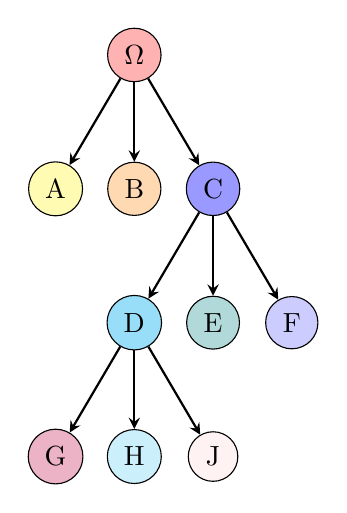
\begin{tikzpicture}[]
    \tikzstyle{space} = [circle, minimum width=1,text centered, draw=black]
    \tikzstyle{arrow} = [thick,->,>=stealth]

    \node(space)[space, fill = red!30]{$\Omega$};

    %depth 1
    \node(B)[space, fill = orange!30, below of = space, yshift = -0.7cm]{B};
    \node(A)[space, fill = yellow!30, left of = B]{A};
    \node(C)[space, fill = blue!40,  right of = B]{C};
    \draw[arrow] (space) -- (A);
    \draw[arrow] (space) -- (B);
    \draw[arrow] (space) -- (C);

    %depth 1
    \node(E)[space, fill = teal!30, below of = C, yshift = -0.7cm]{E};
    \node(D)[space, fill = cyan!40, left of = E]{D};
    \node(F)[space, fill = blue!20,  right of = E]{F};
    \draw[arrow] (C) -- (E);
    \draw[arrow] (C) -- (D);
    \draw[arrow] (C) -- (F);

    %depth 2
    \node(H)[space, fill = cyan!20, below of = D, yshift = -0.7cm]{H};
    \node(G)[space, fill = purple!30, left of = H]{G};
    \node(J)[space, fill = pink!20,  right of = H]{J};
    \draw[arrow] (D) -- (G);
    \draw[arrow] (D) -- (H);
    \draw[arrow] (D) -- (J);


\end{tikzpicture}